\section{Results}\label{sec:results}

We first place SpatialNet against published models and simple references (Section~\ref{sec:main}) and against compact detectors trained under our protocol (Section~\ref{sec:detectors}). We then analyse where it fails (Section~\ref{sec:heads-results}), what input resolution and each component contribute (Sections~\ref{sec:resolution} and~\ref{sec:ablations}), how it behaves with other hands in view (Section~\ref{sec:own}), what it costs on the glasses (Section~\ref{sec:ondevice}) and how it does on frames from their camera (Section~\ref{sec:realframes}). Throughout, the aim is to characterise the operating point, not to claim a more accurate localiser.

SpatialNet numbers are from the seed-42 run, the model deployed on the glasses. Two more seeds (1 and 2) measure how much retraining alone changes the results. P@0.5 is 58.9--59.0\% in all three runs, and P@0.7 and mIoU vary by under 0.8 points. Large-gap targets (25.4--27.8\%) and the median direction error (18.6--20.2$^\circ$) vary more, and small targets vary most (27.8--36.9\%; only 309 test images have one, and seed 42 is the highest of the three). We use this spread to calibrate the single-run comparisons below.

\subsection{Pointed-Target Localisation}\label{sec:main}

We copy published results and do not re-run those models. VistaRef~\cite{li2026vistaref} and PointVG-R~\cite{li2026pointvgr} report results on the same 3,072-image test split, from which ours omits 43 unclear images and the 425 images without a target; PointVG-R also reports zero-shot and fine-tuned multimodal LLMs on that split. EgoPoint-Ground's pointing-only (POG) results~\cite{egopoint} come from a different setting: zero-shot models receive the ground-truth hand box, and the evaluated subset is not stated. Three simple references test whether knowing where the fingertip is would be enough: the mean training target box at a fixed position, and a box of mean training size centred on SpatialNet's predicted fingertip or on the ground-truth fingertip.

\begin{table}[t]
  \caption{Localisation of the pointed-at target on the EgoPoint test split. All columns compare a predicted \emph{target} box with the labelled target box; hand accuracy is in Table~\ref{tab:heads}. Our rows use the 2,604 test images with a target; the 425 no-hand images have none. mIoU and P@$\tau$ (Section~\ref{sec:metrics}) in \%, the published values multiplied by 100. We count IoU${\geq}\tau$, as does VistaRef; EgoPoint-Ground and PointVG-R count IoU${>}\tau$. \emph{Large gap}: P@0.5 on the 209 large-gap targets. Latency per image on the hardware named in the text; only SpatialNet runs on the glasses. Higher-resolution runs of SpatialNet are in Table~\ref{tab:detectors}.\\
  $^\ast$\,VistaRef~\cite{li2026vistaref}, Table~1, setting ``Train-Real Data Test'', BEiT-3-L backbone (226M parameters with BEiT-3-Base); test set of 3,072 images, which includes no-hand images.\\
  $^\ddagger$\,PointVG-R~\cite{li2026pointvgr}, Table~1, EgoPoint-CoT test set, built on the same 15,455-image release and 3,072-image test split.\\
  $^\dagger$\,EgoPoint-Ground~\cite{egopoint}, Table~4, pointing-only (POG) task: inference only, given the ground-truth hand box; the evaluated data subset is not stated.\\
  How the published works score images without a target is not stated; our rows exclude them. If the published averages counted the 425 no-target images as failures, zero-shot Qwen2.5-VL-7B would reach about 57.8\% P@0.5 and 52.8\% mIoU on the images with a target.}
  \label{tab:main}
  \footnotesize
  \setlength{\tabcolsep}{3.4pt}
  \begin{tabular}{lrrrrrrr}
    \toprule
    Method & Params & P@0.3 & P@0.5 & P@0.7 & mIoU & Large gap & Latency \\
    \midrule
    \multicolumn{8}{l}{\emph{Published, trained on EgoPoint (not re-run)}} \\
    \quad VistaRef$^\ast$, image + fixed prompt & $>$226M & 97.0 & 93.9 & 82.6 & 82.0 & -- & -- \\
    \quad PointVG-R$^\ddagger$, image + instruction, SFT + RL & 7B & 88.1 & 83.6 & 74.5 & 75.7 & -- & -- \\
    \quad Qwen2.5-VL-7B$^\ddagger$, image + instruction, SFT & 7B & 68.7 & 63.6 & 56.7 & 59.8 & -- & -- \\
    \multicolumn{8}{l}{\emph{Published, zero-shot (not re-run)}} \\
    \quad Qwen2.5-VL-7B$^\ddagger$, image + instruction & 7B & 54.2 & 49.8 & 42.9 & 45.5 & -- & -- \\
    \quad Qwen3-VL-8B$^\ddagger$, image + instruction & 8B & 48.1 & 44.5 & 39.0 & 43.0 & -- & -- \\
    \quad SV-CoT$^\dagger$, image + hand box & $>$1B & 69.4 & 63.9 & 55.6 & -- & -- & -- \\
    \quad Qwen3-VL-4B$^\dagger$, image + hand box & 4B & 67.1 & 61.2 & 53.2 & -- & -- & -- \\
    \multicolumn{8}{l}{\emph{Simple references}} \\
    \quad Mean training box, fixed position & 0 & 41.3 & 9.6 & 0.9 & 27.4 & 4.3 & -- \\
    \quad Mean-size box at predicted fingertip & 0.72M & 43.5 & 11.2 & 0.9 & 28.8 & 0.0 & -- \\
    \quad Mean-size box at true fingertip (oracle) & -- & 43.6 & 11.4 & 1.0 & 29.0 & 0.0 & -- \\
    \midrule
    \textbf{SpatialNet} (image only, seed 42) & 0.72M & 78.6 & 58.9 & 31.8 & 53.3 & 25.4 & 60--80\,ms \\
    \quad mean $\pm$ std, 3 seeds & & 78.1{\scriptsize$\pm$0.6} & 59.0{\scriptsize$\pm$0.1} & 31.5{\scriptsize$\pm$0.4} & 52.9{\scriptsize$\pm$0.5} & 26.3{\scriptsize$\pm$1.3} & \\
    \bottomrule
  \end{tabular}
\end{table}

Table~\ref{tab:main} shows, first, that the target head does real work. Knowing the fingertip is not enough: a mean-size box at the true fingertip reaches a P@0.5 of only 11.4\% (12.0\% when shifted by the mean training offset), because target sizes vary widely (2.6\% to 44\% of the image area, 10th to 90th percentile), while SpatialNet reaches 58.9\%.

Second, large models trained on EgoPoint are far more accurate. SpatialNet is 35 points below VistaRef in P@0.5 and 51 points below in P@0.7, where its boxes are least precise (mIoU 53.3 against 82.0). It is 25 points below PointVG-R, and 4.7 points below Qwen2.5-VL-7B fine-tuned on the same data.

Third, against zero-shot multimodal LLMs the picture is mixed. SpatialNet's P@0.5 and mIoU are above those reported for zero-shot Qwen2.5-VL-7B (49.8\% and 45.5\%) and Qwen3-VL-8B (44.5\% and 43.0\%), and its P@0.3 is far higher (78.6\% against 48.1--54.2\%). However, the zero-shot models draw tighter boxes (P@0.7 of 39.0--42.9\% against 31.8\%), and models given the true hand box reach 61.2--63.9\% P@0.5. Because the published rows count IoU${>}\tau$, include no-target images scored in an unstated way and, in one case, use an unstated subset, and because models trained on large image collections may also have seen COCO, the source of at least 41\% of our test images (Section~\ref{sec:data}), we read this as the same accuracy range at a fraction of the size, not as parity or superiority.

\subsection{Compact Detectors at Matched Compute}\label{sec:detectors}

The published models above are 300 to 10{,}000 times larger and were not re-run. Table~\ref{tab:detectors} therefore compares SpatialNet with YOLO26n and NanoDet-Plus-m, which we trained on the same split and scored with the same code (Section~\ref{sec:metrics}). At 0.22--0.23 GFLOPs, these detectors cost about the same compute as SpatialNet at 160\,px; the lower block adds higher-resolution runs of both.

\begin{table}[t]
  \caption{SpatialNet and compact detectors trained on EgoPoint and scored by the same code. Accuracy in \%, on the 2,604 test images with a target, except \emph{End-to-end}, which covers all 3,029 test images and also counts missed hands and false alarms (Section~\ref{sec:metrics}). Model names give the input size and the pretraining of the backbone. \emph{Large gap}: P@0.5 on the 209 large-gap targets. \emph{Centre in}: predicted target centre inside the labelled box. \emph{Pasted}: change in target P@0.5 when one or two hands are pasted into each test image (Section~\ref{sec:own}); none of these detectors was trained with pasted hands, and Table~\ref{tab:controlled} adds one that was. Bold: best among the matched-compute models without COCO data. $^\dagger$\,Pretrained on COCO train2017, which contains the source photographs of at least 41\% of the test images (Section~\ref{sec:data}); the controlled runs of Table~\ref{tab:controlled} find no extra gain on those images. Paired intervals for the main comparisons are in Table~\ref{tab:controlled} and the text.}
  \label{tab:detectors}
  \footnotesize
  \setlength{\tabcolsep}{3pt}
  \begin{tabular}{lrrrrrrrrrr}
    \toprule
    Model & Params & GFLOPs & P@0.5 & P@0.7 & mIoU & Large & Hand & Centre & Pasted & End-to- \\
    & & & & & & gap & mIoU & in & & end \\
    \midrule
    \multicolumn{11}{l}{\emph{Matched compute, no COCO data}} \\
    \textbf{SpatialNet}, 160\,px, ImageNet & \textbf{0.72M} & 0.231 & 58.9 & 31.8 & 53.3 & 25.4 & 73.7 & \textbf{84.8} & \textbf{$+$1.2} & 63.6 \\
    YOLO26n, 128\,px, scratch & 2.50M & 0.225 & 59.9 & 39.1 & 54.7 & 31.6 & 80.6 & 81.6 & $-$4.6 & 63.8 \\
    YOLO26n, 128\,px, ImageNet & 2.50M & 0.225 & \textbf{63.2} & \textbf{42.4} & \textbf{56.8} & \textbf{36.8} & \textbf{81.1} & 82.3 & $-$3.6 & \textbf{67.4} \\
    \multicolumn{11}{l}{\emph{Matched compute, COCO-pretrained}$^\dagger$} \\
    YOLO26n, 128\,px, COCO$^\dagger$ & 2.50M & 0.225 & 65.0 & 47.0 & 58.6 & 39.7 & 81.6 & 82.2 & $-$4.0 & 68.9 \\
    NanoDet-Plus-m, 160\,px, COCO$^\dagger$ & 1.17M & 0.218 & 67.6 & 49.5 & 59.8 & 40.7 & 81.5 & 82.9 & $-$4.5 & 71.1 \\
    \midrule
    \multicolumn{11}{l}{\emph{Higher compute}} \\
    SpatialNet, 224\,px, ImageNet & 0.72M & 0.453 & 62.4 & 37.1 & 54.8 & 35.9 & 74.9 & 83.7 & $+$1.5 & 66.8 \\
    SpatialNet, 320\,px, ImageNet & 0.72M & 0.923 & 65.1 & 40.3 & 56.5 & 34.9 & -- & -- & -- & 69.3 \\
    YOLO26n, 160\,px, COCO$^\dagger$ & 2.50M & 0.352 & 66.9 & 48.8 & 60.3 & 42.1 & 82.1 & 83.5 & $-$3.0 & 70.8 \\
    YOLO26n, 192\,px, COCO$^\dagger$ & 2.50M & 0.507 & 69.9 & 53.3 & 62.8 & 43.5 & 82.9 & 84.7 & $-$2.6 & 73.6 \\
    \bottomrule
  \end{tabular}
\end{table}

\paragraph{At the same compute, the detectors draw better boxes, even without COCO data.} With the same ImageNet pretraining as our backbone, YOLO26n is 4.3 points ahead in P@0.5, mostly in tight boxes (P@0.7 +10.6) and large-gap targets (+11.4), and its hand mIoU is 7.4 points higher; trained from scratch, it is 1.0 point ahead. The COCO-pretrained detectors score higher still (YOLO26n 65.0\%, NanoDet-Plus-m 67.6\%).

\paragraph{Controlled runs.} To test these comparisons with paired intervals, and to answer two questions that Table~\ref{tab:detectors} leaves open, we trained YOLO26n four more times under one recipe, scored with the same code and on the same images as SpatialNet (Section~\ref{sec:metrics}): with an ImageNet start (two seeds), with an ImageNet start and our distractor pasting, and with a COCO start (Table~\ref{tab:controlled}). The ImageNet-start run reproduces the benchmark (62.9\% against 63.2\% P@0.5), and its second seed differs from it by 0.6 points ([$-$1.0, +2.2]). Against the first seed, SpatialNet is 4.0 points lower in P@0.5 ([$-$6.0, $-$2.2]) and 11.6 lower in P@0.7 ([$-$13.4, $-$9.6]); against the second, 4.6 and 11.5 points lower.

\begin{table}[t]
  \caption{SpatialNet and four controlled YOLO26n runs (128\,px), scored by the same code on the same test images. The ImageNet start was trained with two seeds, the other starts once; the seed-42 ImageNet-start row reproduces the corresponding row of Table~\ref{tab:detectors} within 0.3 points of P@0.5. Accuracy in \%, on the 2,604 test images with a target. \emph{Pasted}: change in target P@0.5 with one or two pasted hands per image (the seed-42 set of Section~\ref{sec:own}). \emph{No hand kept}: no-hand images still classed as no hand when hands are pasted into them; the hand-gate threshold of every model, SpatialNet included, is tuned on the validation split, so SpatialNet's value differs from Table~\ref{tab:own}. \emph{COCO} and \emph{Other}: P@0.5 on the 842 test images made from COCO train2014 photographs and on the remaining 1,762. \emph{+ pasting}: trained with our distractor-hand pasting. Paired 95\% intervals are in the text.}
  \label{tab:controlled}
  \footnotesize
  \setlength{\tabcolsep}{2.6pt}
  \begin{tabular}{lrrrrrrrrr}
    \toprule
    & & & Large & Hand & Centre & & No hand & \multicolumn{2}{c}{P@0.5, source} \\
    \cmidrule(l){9-10}
    Model & P@0.5 & P@0.7 & gap & mIoU & in & Pasted & kept & COCO & Other \\
    \midrule
    \textbf{SpatialNet} (ImageNet) & 58.9 & 31.8 & 25.4 & 73.7 & \textbf{84.8} & $+$1.2 & 96.7 & 51.8 & 62.3 \\
    YOLO26n, ImageNet & 62.9 & 43.4 & 36.8 & 81.0 & 82.1 & $-$3.1 & 87.8 & 56.1 & 66.2 \\
    YOLO26n, ImageNet, seed 1 & 63.6 & 43.3 & 38.3 & 81.0 & 81.6 & $-$4.1 & 88.7 & 54.9 & 67.7 \\
    YOLO26n, ImageNet + pasting & 63.2 & 42.7 & 36.8 & 80.9 & 81.8 & $+$0.7 & 95.8 & 55.5 & 66.9 \\
    YOLO26n, COCO & 64.4 & 45.5 & 36.4 & 81.4 & 82.2 & $-$2.4 & 87.8 & 55.3 & 68.7 \\
    \bottomrule
  \end{tabular}
\end{table}

\paragraph{SpatialNet picks the labelled object more often.} Its predicted target centre lies inside the labelled box in 84.8\% of images, against 81.6--82.2\% for the four controlled detectors; the paired differences are 2.8 [1.4, 4.1] and 3.2 [1.8, 4.6] points against the two ImageNet-start seeds, 3.0 [1.7, 4.5] against the run with pasting and 2.6 [1.3, 4.0] against the COCO start. Together with the error analysis of Section~\ref{sec:heads-results}, this locates SpatialNet's deficit in box extent rather than in which object it picks.

\paragraph{For naming the target, the detectors' tighter boxes do not help.} Better target choice and tighter boxes pull in opposite directions, so we measured which one matters when a ``what is that?'' assistant classifies the crop (Section~\ref{sec:metrics}; Table~\ref{tab:recog}). With both recognisers, SpatialNet's crops are named correctly as often as the detectors' crops: the paired differences in top-1 accuracy range from $-$1.3 to $+$0.3 points, and every 95\% interval includes zero and lies between $-$2.8 and $+$1.8 points. Top-5 accuracy gives the same result (differences from $-$1.3 to 0.0 points; one interval of eight excludes zero, by 0.04 points), and so do seeds 1 and 2 of SpatialNet (48.3--49.1\% and 52.5--52.6\% top-1). Localising the target is worth it: SpatialNet's crops are named correctly 6--8 points more often than the whole frame and reach 88--90\% of the rate for crops of the labelled box. The reason is the error type found in Section~\ref{sec:heads-results}. When SpatialNet's box misses IoU 0.5 but its centre lies on the labelled object, as in 26\% of images, the crop is still named correctly in 47--51\% of them, close to the 54--58\% for boxes with IoU${\geq}0.5$ and well above the 30\% when the centre misses. Large-gap targets are the exception: there, the detectors' crops are named correctly 4.3--8.1 points more often than those of the deployed model (the interval excludes zero in five of the eight comparisons; seeds 1 and 2 lie in between, at 37.3--43.1\%), and its crops are named about as often as the whole frame, or less often (34.9 and 36.8\% against 33.5 and 43.1\%). Restricting the test to targets other than people, 20\% of the test set, changes no difference by more than one point.

\begin{table}[t]
  \caption{Downstream recognition: how often an off-the-shelf zero-shot recogniser names the labelled category from a crop of each model's target box, choosing among the 348 EgoPoint category names (top-1 accuracy in \%; 2,603 test targets, 209 of them with a large gap). The labelled box and the whole frame are references. Category-level test: a box on a neighbouring object of the same category counts as correct. Paired differences are in the text.}
  \label{tab:recog}
  \footnotesize
  \begin{tabular}{lrrrr}
    \toprule
    & \multicolumn{2}{c}{CLIP ViT-B/16} & \multicolumn{2}{c}{SigLIP base} \\
    \cmidrule(lr){2-3}\cmidrule(l){4-5}
    Crop & All & Large gap & All & Large gap \\
    \midrule
    Labelled box (upper reference) & 53.9 & 51.2 & 59.4 & 54.1 \\
    Whole frame (lower reference) & 40.3 & 33.5 & 46.2 & 43.1 \\
    \midrule
    \textbf{SpatialNet} (seed 42) & 48.6 & 34.9 & 52.3 & 36.8 \\
    YOLO26n, ImageNet & 48.8 & 43.1 & 53.3 & 41.6 \\
    YOLO26n, ImageNet, seed 1 & 49.1 & 41.1 & 53.4 & 41.1 \\
    YOLO26n, ImageNet + pasting & 49.9 & 43.1 & 52.0 & 43.5 \\
    YOLO26n, COCO & 49.1 & 42.1 & 53.2 & 42.1 \\
    \bottomrule
  \end{tabular}
\end{table}

\paragraph{Robustness to other hands comes from the training recipe, and the recipe transfers.} Trained without pasting, the detectors lose 2.4--4.1 points of P@0.5 when hands are pasted into the test images and keep only 87.8--88.7\% of no-hand frames, whereas SpatialNet gains 1.2 points and keeps 96.7\%. Trained with our pasting, the same YOLO26n is as stable as SpatialNet: it changes by $+$0.7 points (difference from SpatialNet $-$0.6 [$-$2.2, $+$0.8]) and keeps 95.8\% of no-hand frames ($-$0.9 [$-$3.8, $+$1.4]). Pasting improves the detector's change under interference by 3.8 points [2.4, 5.2] and the no-hand frames kept by 8.0 [5.2, 10.8], at no cost on clean images (P@0.5 $+$0.3 [$-$1.2, $+$1.8]). The robustness therefore comes from the distractor-pasting recipe, not from SpatialNet's architecture, and the recipe carries over unchanged to a generic detector.

\paragraph{No sign that the COCO overlap inflates the COCO-pretrained detector.} If COCO pretraining helped mainly by having seen the test sources, its gain would concentrate on the 842 COCO-derived test images. It does the opposite: against the ImageNet start, the COCO start gains 2.4 points [0.6, 4.3] on the other test images and $-$0.7 [$-$3.7, $+$2.5] on the COCO-derived ones (difference $-$3.2 [$-$6.7, $+$0.3]). The gain from COCO pretraining is therefore general transfer rather than recall of the test sources. NanoDet-Plus-m was not retrained, so this test covers YOLO26n only. All models, SpatialNet included, find the COCO-derived images harder (51.8--56.1\% against 62.3--68.7\% P@0.5).

\paragraph{The end-to-end score preserves the ranking.} Counting the hand gate costs each model 0.3--1.3 points of P@0.5, and with validation-tuned thresholds every model rejects 95.3--98.4\% of no-hand frames, so the order does not change: SpatialNet reaches 63.6\%, on a par with YOLO26n from scratch (63.8\%) and below YOLO26n with an ImageNet start (67.4\%) and the COCO-pretrained detectors (68.9--71.1\%). On the test split without duplicates, the order is the same (SpatialNet 62.4\%; detectors at matched compute 62.9--70.1\%).

\paragraph{What the detectors' lead means.} For an application that needs a tight target box, a compact detector trained on EgoPoint is the more accurate choice at this compute, even without COCO pretraining, and our pasting recipe makes it as robust to other hands as SpatialNet; this is itself useful guidance for wearable designers. For naming the target, the detectors' box precision does not show, except for large-gap targets. SpatialNet also picks the labelled object more often and returns the hand, fingertip and direction from the same pass, with fewer parameters (0.72M and 1.6\,MB in FP16, against 1.17M and 2.4\,MB for NanoDet-Plus-m and 2.50M and 4.8\,MB for YOLO26n). An interface can use these outputs for feedback, such as drawing the ray or a fingertip cursor, which helps mid-air pointing~\cite{mayer2018effect}, and for hand-presence gating; whether users benefit from them, we did not evaluate. We also did not measure the detectors' latency on the glasses, and a detector with an added keypoint head, which could output the fingertip too, remains to be tested.

\subsection{Per-Head Accuracy and Fingertip--Target Gap}\label{sec:heads-results}

Table~\ref{tab:heads} breaks the result down by head and by fingertip--target gap; IoU success curves are in Appendix~\ref{app:extra}.

\begin{table}[t]
  \caption{Accuracy of each head by fingertip--target gap (test split, pointing-at-target images). Fingertip error in pixels at the $160\times160$ input; direction error in degrees. mIoU and P@0.5 in \%; brackets: 95\% bootstrap confidence intervals of the mIoU.}
  \label{tab:heads}
  \footnotesize
  \setlength{\tabcolsep}{4pt}
  \begin{tabular}{lrrrrrrrr}
    \toprule
    & \multicolumn{2}{c}{Hand} & \multicolumn{2}{c}{Fingertip (px)} & \multicolumn{2}{c}{Direction ($^\circ$)} & \multicolumn{2}{c}{Target} \\
    \cmidrule(lr){2-3}\cmidrule(lr){4-5}\cmidrule(lr){6-7}\cmidrule(l){8-9}
    Gap (images) & mIoU & P@0.5 & mean & ${<}5$\,px & mean & ${<}15^\circ$ & mIoU [CI] & P@0.5 \\
    \midrule
    Overlap (1,796) & 73.7 & 92.3 & 3.79 & 84.4 & 36.0 & 39.7 & 57.9 [56.8, 59.0] & 66.0 \\
    Near (599) & 73.7 & 93.5 & 4.09 & 78.8 & 22.0 & 54.9 & 47.8 [45.8, 49.8] & 49.2 \\
    Large gap (209) & 72.7 & 92.8 & 4.16 & 80.9 & 29.0 & 36.8 & 29.8 [26.0, 33.6] & 25.4 \\
    \midrule
    All (2,604) & 73.7 & 92.6 & 3.89 & 82.8 & 32.2 & 43.0 & 53.3 [52.3, 54.3] & 58.9 \\
    \bottomrule
  \end{tabular}
\end{table}

\paragraph{Hand presence.} The hand gate separates no-hand from pointing frames with 98.6\% accuracy (95\% CI 98.1--98.9) and AUROC 0.998. At threshold 0.5, it misses 15 of 2,604 hands (0.6\%) and raises false alarms on 28 of 425 no-hand frames (6.6\%). Choosing the threshold on validation so that no hand is missed (0.22) would raise false alarms to 117 (27.5\%), so we keep 0.5; the validation-tuned threshold of the end-to-end score gives 97.2\% correct no-hand frames. Per-frame false alarms of this size mean that an always-on interface needs temporal smoothing, for example requiring several consecutive detections, which we do not evaluate.

\paragraph{Where the errors come from.} The hand box and fingertip are equally good at every gap (hand P@0.5 of 92--94\%; about 4\,px fingertip error, 2.5\% of the image side), so they are not the bottleneck. The target falls off with the gap: P@0.5 drops from 66.0\% for overlap targets to 49.2\% for near and 25.4\% for large-gap ones (mIoU from 57.9 to 47.8 and 29.8). The direction is coarse: its median error is 18.6$^\circ$, and only 36.8\% of large-gap targets have an error below 15$^\circ$. At their median fingertip--target distance of 0.32 image widths, 15$^\circ$ already moves the ray by about 0.08 image widths, the size of a small object. The error is largest for overlap targets (36$^\circ$), where the direction to the target centre is ill-defined and matters least. Finally, position and extent errors contribute about equally. The predicted target centre lies inside the labelled box in 84.8\% of images; giving the model the true size with its own centre would raise P@0.5 to 70.4\%, and giving it the true centre with its own size would raise it to 72.3\%. Size is regressed towards the mean: small targets (under 3\% of the image) are predicted about 1.9 times too large and reach a P@0.5 of only 36.9\% (27.8--36.9\% across seeds).

\subsection{Input Resolution}\label{sec:resolution}

A convolutional network shares its filters across positions, so a larger input costs compute but no parameters. We retrained the unchanged model (722,104 parameters, same seed and settings) at 224\,px, using the stored $224\times224$ images at full resolution instead of downsampling them, and at 320\,px, re-converting the dataset from the original images so that the larger input carries real detail rather than upsampled pixels. The lower block of Table~\ref{tab:detectors} lists the results.

Resolution is the largest lever we found, at no parameter cost. From 160 to 320\,px, P@0.5 rises by 6.2 points (95\% paired-bootstrap CI [+4.4, +8.0]) to 65.1\%, P@0.7 by 8.5 points [+6.8, +10.3] and mIoU by 3.2, and the fingertip error falls from 2.43\% to 1.32\% of the image width; 224\,px lies in between (P@0.5 62.4\%, fingertip error 1.81\%). Each doubling of compute adds 2.7--3.5 points of P@0.5, far more than the 0.1-point spread between seeds. Large-gap targets gain first and then stop: their P@0.5 rises from 25.4\% to 35.9\% at 224\,px (+10.5, CI [+4.3, +16.8]) and is 34.9\% at 320\,px, while the mean direction error is flat at every resolution (31.4--32.2$^\circ$). With one run per resolution, this suggests, but does not show, that the direction estimate rather than the input limits large-gap targets beyond 224\,px. Small targets gain only at 320\,px (36.9\% $\to$ 46.6\% P@0.5, +9.7, CI [+4.2, +15.2]), where the images were re-converted from the originals and carry detail that the stored 224\,px images lack.

Both higher-resolution runs stopped early at 84 epochs (best epoch 59, against 100 at 160\,px), so their gains may be underestimated. The validation loss is not comparable across resolutions, because the heatmap terms sum over more cells, which also makes early stopping trigger sooner. Compute grows from 0.23 to 0.45 and 0.92 GFLOPs (CPU latency on the evaluation machine 25.7, 37.2 and 50.8\,ms), while the weights stay at 1.6\,MB. We deploy the 160\,px model, the one measured on the glasses; the 224 and 320\,px results quantify how much accuracy is available to a device that can afford two to four times the compute.

\subsection{Ablations: What Each Component Buys}\label{sec:ablations}

Each component of SpatialNet was added for a specific purpose. We retrain the 160\,px model without one component at a time, with the seed and settings of the main run:
\begin{itemize}
\item \textbf{A1} no distractor pasting and no ownership weighting;
\item \textbf{A2} no geometric consistency terms ($\mathcal{L}_{\mathrm{ray}}$ and the hand-axis term);
\item \textbf{A3} no ray conditioning of the target head (no $G^t$; 13,105 fewer parameters);
\item \textbf{A4} no instance-anchored chain: the direction head and gates read the globally pooled vector, and the fingertip has no hand-anchored terms, which gives a plain model of the same size (709K parameters).
\end{itemize}
Each ablation was trained once, and we test each difference in two ways. A paired bootstrap over test images (resampling the images and recomputing the difference on the same images) gives a 95\% confidence interval for test-sample variation, and retraining the full model with two more seeds gives the training variation. A difference counts as an effect only if its interval excludes zero \emph{and} it exceeds the largest change that retraining alone produced (Table~\ref{tab:ablation}, second row). Table~\ref{tab:ablation} reports every metric for every ablation, and Figure~\ref{fig:ablation} shows, for each component, the metrics it was designed to improve. With one seed per variant and several metrics per component, we treat these comparisons as exploratory.

\begin{table}[t]
  \caption{Ablations at 160\,px (one seed each). First row: the full model's values; other rows: difference from the full model (points, or degrees for the direction error, where positive means worse). \emph{Retraining}: the largest difference of seeds 1 and 2 from seed 42, i.e.\ what retraining the full model alone changes. Bold: the 95\% paired-bootstrap interval excludes 0 and the difference exceeds the retraining row. $^\S$\,Not significant on the duplicate-free test split (Section~\ref{sec:data}). \emph{Large gap}: P@0.5 on large-gap targets. \emph{Small}: targets under 3\% of the image (309 images). \emph{With other hands}: test images with one or two pasted hands (Section~\ref{sec:own}).}
  \label{tab:ablation}
  \footnotesize
  \setlength{\tabcolsep}{3pt}
  \begin{tabular}{lrrrrrrrrr}
    \toprule
    & \multicolumn{7}{c}{Clean test images} & \multicolumn{2}{c}{With other hands} \\
    \cmidrule(lr){2-8}\cmidrule(l){9-10}
    Variant & mIoU & P@0.5 & P@0.7 & Large gap & Small & Hand & Dir.\,($^\circ$) & P@0.5 & No hand \\
    \midrule
    Full model & 53.3 & 58.9 & 31.8 & 25.4 & 36.9 & 73.7 & 32.2 & 60.1 & 91.8 \\
    \quad Retraining (seeds 1, 2) & $\pm$0.9 & $\pm$0.1 & $\pm$0.8 & $\pm$2.4 & $\pm$9.1 & $\pm$0.3 & $\pm$1.2 & $\pm$0.4 & $\pm$3.3 \\
    \midrule
    A1 no hand pasting & \textbf{$-$1.2} & $-$0.1 & $-$1.3 & $+$1.9 & $-$3.9 & \textbf{$-$0.6} & \textbf{$+$1.8} & \textbf{$-$4.1} & \textbf{$-$5.4} \\
    A2 no ray / axis losses & $-$0.5 & $+$1.1 & $+$0.6 & $+$3.3 & $-$0.6 & $-$0.4 & \textbf{$+$1.5} & 0.0 & $-$1.2 \\
    A3 no ray conditioning & $+$0.2 & $+$0.7 & \textbf{$+$1.9}$^\S$ & $+$5.3 & $+$1.0 & 0.0 & \textbf{$-$1.3} & $+$1.0 & $+$1.2 \\
    A4 no anchor chain & \textbf{$-$1.4} & $-$0.3 & \textbf{$-$2.8}$^\S$ & $+$0.5 & \textbf{$-$11.3} & \textbf{$-$1.8} & \textbf{$+$3.4} & $-$0.5 & 0.0 \\
    \bottomrule
  \end{tabular}
\end{table}

\begin{figure}[t]
  \centering
  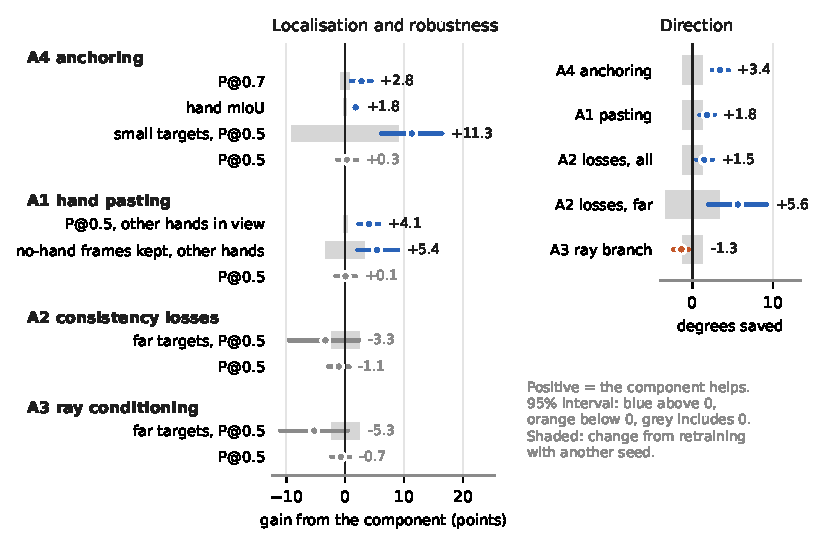
\includegraphics[width=\linewidth]{figures/ablation_effects}
  \caption{What each component contributes, with 95\% paired-bootstrap intervals. Gain = full model minus ablation, or degrees of direction error saved, so positive means the component helps. Grey bands: the largest change that retraining the full model with another seed produced on the same metric. For each component, the first rows show the capability it was designed for and the last row shows P@0.5. ``Far'' in the labels denotes large-gap targets. The P@0.7 effect of A4 is not significant on the duplicate-free test split (Table~\ref{tab:ablation}).}
  \Description{Interval plot with grey bands for retraining variation. Anchoring: P@0.7 +2.8, hand mIoU +1.8, small targets +11.3, all above zero and outside the bands; P@0.5 +0.3, crossing zero. Hand pasting: P@0.5 with other hands +4.1 and no-hand frames kept +5.4, above zero; P@0.5 +0.1. Consistency losses and ray conditioning: far-target and overall P@0.5 effects cross zero. Direction panel: degrees saved by anchoring 3.4, pasting 1.8, consistency losses 1.5 overall and 5.6 for far targets, all above zero; the ray branch -1.3, below zero.}
  \label{fig:ablation}
\end{figure}

\paragraph{No component changes coarse accuracy.} All four variants stay within ${\pm}1.1$ points of the full model's P@0.5 (58.9\%), and none differs significantly; retraining alone moves P@0.5 by 0.1 points, so we draw no conclusions from P@0.5 differences. The components differ instead in the capabilities they add, at a cost of at most 13K parameters each.

\paragraph{A4, instance anchoring: a more precise hand box and direction.} Against a plain model of the same size, the anchored chain improves hand mIoU by 1.8 points [+1.4, +2.2], against at most 0.3 between seeds, and lowers the direction error by 3.4$^\circ$ [2.4, 4.5], against at most 1.2$^\circ$. It also raises P@0.7 by 2.8 points [+1.1, +4.3] and small-target P@0.5 by 11.3 points [+6.5, +16.5] (the plain model's small boxes are drawn 2.4 instead of 1.9 times too large), but we treat these two as supporting evidence only: without duplicated test images the P@0.7 gain shrinks to 1.7 [0.0, +3.5], and the small-target gain is close to the seed spread (9.1). A plain model therefore finds the right region as often, but with a less precise hand box and direction. A4 also stopped earliest (best epoch 54, against 100), so its effects include a different training length.

\paragraph{A1, distractor pasting: robustness to synthetic other hands.} With other hands in view, the model trained with pasting keeps 4.1 more points of target P@0.5 [+2.4, +5.8] and 5.4 more points of no-hand frames as \emph{no hand} [+1.9, +8.9], and it puts its hand on another person's hand six times less often (0.2\% against 1.2\%). On clean images it costs nothing (P@0.5 $-$0.1) and even helps slightly (mIoU +1.2, hand mIoU +0.6, and 1.8$^\circ$ less direction error), which is consistent with pasting acting as a regulariser that makes the model rely on the hand's position and context rather than on its appearance alone. The ownership-accuracy metric itself barely moves (99.7\% against 98.7\%), because pasted hands sit higher in the frame than the wearer's (Section~\ref{sec:own}).

\paragraph{A2, consistency losses: a sharper direction, not a better box.} Without the two consistency terms, the direction error for large-gap targets rises by 5.6$^\circ$ [+2.1, +9.4], to 34.6$^\circ$, above all three seeds of the full model (29.0--32.3$^\circ$); this is where the ray-alignment term weighs most. Overall, the direction error rises by 1.5$^\circ$, only slightly more than retraining alone changes it (1.2$^\circ$). Target-box accuracy does not change ($+$1.1 P@0.5, n.s.), because the target head does not draw on the predicted direction (A3 below). The losses therefore sharpen an output that an interface can use directly, for example to draw the pointing ray as feedback, but not the box.

\paragraph{A3, explicit ray geometry: what a small model learns from it.} Removing the ray branch $G^t$ changes P@0.5 by less than one point ($+$0.7, n.s.). P@0.7 rises by 1.9 points [+0.2, +3.6] and the direction error falls by 1.3$^\circ$, both outside the seed spread, but the P@0.7 gain does not survive the duplicate check ($+$1.6 [$-$0.2, +3.3]), and A3 also trained 20\% longer (best epoch 120). Probing the trained full model suggests why the branch adds nothing. The model does rely on it: its output is as large as the visual term (median ratio of spreads 0.86 on 500--800 test images), and switching it off at inference lowers P@0.5 on the whole test split from 58.9\% to 50.6\%. But it has learned proximity more than direction: its output correlates more with closeness to the fingertip ($\rho=-0.38$) than with closeness to the ray's line ($-0.27$), and on the probe subset hardly at all with being in front of the fingertip ($+0.04$). Accordingly, switching it off costs 11 points of P@0.5 on overlap targets and 9.5 on near ones in the probe subset, while on large-gap targets of the whole test split P@0.5 even rises by 2.0 points. A plausible reason is the training distribution: with 70\% overlap and 7\% large-gap targets, a ``near the fingertip'' prior already fits most targets, and the visual head can learn it by itself. The branch can therefore be dropped without loss. We keep it in the deployed model because that is the model measured on the glasses. The next paragraph tests the two remedies this analysis suggests.

\paragraph{Testing the remedies.} We retrained the 160\,px model three more times, each with one change and the seed and settings of the main run (Table~\ref{tab:remedies}). E1 lets the learned ray prior act only in front of the fingertip ($G^t$ is set to zero wherever $t_k<0$). E2 weights the target-box and target-heatmap losses three times as much for near and large-gap targets, the 30\% of training images in which the fingertip does not overlap the target. E3 spaces the $3\times3$ sample that predicts the target size two cells apart, so that it covers 40 instead of 24 pixels; none of the three adds a parameter.
\begin{itemize}
\item \emph{Neither remedy for large-gap targets works.} Constraining the prior to point forward (E1) leaves P@0.5 unchanged; large-gap P@0.5 rises by 5.3 points, but the interval includes zero ([$-$0.5, +11.0]), and the direction error for large-gap targets grows by 4.3$^\circ$. Up-weighting non-overlap targets (E2) trades overlap accuracy for gains that are not significant: overlap P@0.5 falls by 3.8 points and overall P@0.5 by 1.8, while near and large-gap P@0.5 rise by 2.0 and 3.8 points with intervals that include zero; the hand box and the overall direction also become less precise (hand mIoU $-$1.2, direction error $+$2.5$^\circ$).
\item \emph{A wider size sample does not tighten the boxes.} With the size sample spaced two cells apart (E3), P@0.7 changes by $-$1.2 points and small-target P@0.5 by $+$1.3, both with intervals that include zero, while the hand box and the large-gap direction become slightly less precise. Box extent is therefore not limited by how far the size head looks around the predicted centre; a different size head, closer to the multi-scale box regression of detectors, is left to future work.
\end{itemize}
Together with A2, A3 and the flat direction error across resolutions, these results locate the remaining bottleneck for large-gap targets in how the direction is estimated, not in how the ray prior is shaped or how the training images are weighted. A direction supervised by the finger's own axis, for example from finger keypoints, remains untested.

\begin{table}[t]
  \caption{Remedies tested at 160\,px (one seed each; no extra parameters). Differences from the full model, in points (degrees for the direction error, where positive means worse); brackets: 95\% paired-bootstrap interval. Bold: the interval excludes 0 and the difference exceeds the largest change between the three seeds of the full model (P@0.5 0.1, P@0.7 0.8, overlap 0.5, large gap 2.4, small 9.1, hand mIoU 0.3, large-gap direction 3.4$^\circ$). Best epoch in parentheses (full model: 100).}
  \label{tab:remedies}
  \footnotesize
  \setlength{\tabcolsep}{2.5pt}
  \begin{tabular}{lrrrrrrr}
    \toprule
    Variant & P@0.5 & P@0.7 & Overlap & Large gap & Small & Hand mIoU & Dir.\ large gap ($^\circ$) \\
    \midrule
    Full model & 58.9 & 31.8 & 66.0 & 25.4 & 36.9 & 73.7 & 29.0 \\
    \midrule
    E1 forward-only ray prior (78) & $+$0.3 & $+$0.2 & $-$0.4 & $+$5.3 {\scriptsize[$-$0.5, +11.0]} & $-$4.2 & \textbf{$-$0.8} & \textbf{$+$4.3} \\
    E2 non-overlap targets $\times3$ (65) & \textbf{$-$1.8} & \textbf{$-$3.7} & \textbf{$-$3.8} & $+$3.8 {\scriptsize[$-$1.9, +9.6]} & $-$3.6 & \textbf{$-$1.2} & $-$0.8 \\
    E3 size sample spaced 2 cells (82) & $+$0.2 & $-$1.2 & $-$0.8 & $+$3.4 {\scriptsize[$-$2.4, +9.6]} & $+$1.3 & \textbf{$-$0.6} & \textbf{$+$3.7} \\
    \bottomrule
  \end{tabular}
\end{table}

\paragraph{Robustness of these conclusions.} Every difference reported above as an effect is significant under the paired bootstrap and larger than the change produced by retraining with another seed; effects close to that threshold (the small-target gain of anchoring, and the overall direction changes of A1--A3, 1.3--1.8$^\circ$ against 1.2$^\circ$) are supporting evidence only. Removing duplicated test images changes no conclusion except the P@0.7 effects of A3 and A4. The loss weights were not searched (Appendix~\ref{app:weights}); A2 covers the two non-standard terms, and the remaining eleven are standard box, keypoint, heatmap and focal losses. Finally, replacing the backbone with MobileNetV3-Small~\cite{howard2019mobilenetv3} or MobileNetV4-Conv-Small~\cite{qin2024mobilenetv4} does not change P@0.5 significantly while doubling or nearly tripling the parameters (Appendix~\ref{app:extra}), so ShuffleNetV2 0.5$\times$ is the efficient choice at this scale.

\subsection{Other People's Hands in View}\label{sec:own}

With one or two pasted hands in each test image (Table~\ref{tab:own}), the model's hand still lies nearer the wearer's hand than any pasted hand in 99.7\% of hand images, and target P@0.5 does not drop (60.1\% against 58.9\% on clean images). This ownership metric is easy under the synthetic distribution: pasted hands sit in the upper part of the frame and the wearer's hand in the lower part, so ownership accuracy on training batches was already 93\% in the first epoch, when the hand IoU was only 0.38. Two numbers are more informative. Pasted hands rarely turn a no-hand frame into a hand frame: 91.8\% of no-hand frames stay \emph{no hand}, against 93.4\% without pasted hands. And the training recipe is needed: without it (A1), target P@0.5 with other hands in view drops by 4.1 points and no-hand frames kept drop by 5.4, while clean accuracy is unchanged. The compact detectors of Section~\ref{sec:detectors}, trained without pasting, lose 2.4--4.6 points under the same pasted hands, but YOLO26n trained with our pasting is as stable as SpatialNet (Table~\ref{tab:controlled}): the robustness to synthetic other hands comes from the training recipe and transfers to a generic detector. EgoPoint contains no real frames with other people's hands, and we did not record any, so robustness to real bystander hands remains untested.
%% Optional, only if part G3 of the device request (companions' hands in view) comes back: add the ownership
%% accuracy on those frames here, with a Wilson interval and Cohen's kappa, and a row to Table tab:own.

\begin{table}[t]
  \caption{Ownership on test images with one or two pasted hands. All values in \%. \emph{On other hand}: predicted hand centre inside a pasted hand. \emph{No hand kept}: no-hand images still classed as no hand, at the hand-gate threshold of 0.5.}
  \label{tab:own}
  \footnotesize
  \begin{tabular}{lrrrr}
    \toprule
    & Ownership accuracy & On other hand & No hand kept & Target P@0.5 \\
    \midrule
    Full model, clean test images & -- & -- & 93.4 & 58.9 \\
    Full model, pasted hands & 99.7 [99.4, 99.9] & 0.2 & 91.8 & 60.1 \\
    A1 (no pasting), pasted hands & 98.7 [98.2, 99.1] & 1.2 & 86.4 & 56.1 \\
    \bottomrule
  \end{tabular}
\end{table}

\subsection{On-Device Performance}\label{sec:ondevice}

Table~\ref{tab:device} reports cost on the evaluation machine and on the glasses.

\begin{table}[t]
  \caption{Inference cost of the 160\,px model. Server rows: PyTorch eager mode, batch size 1, on the 4-core Kaggle virtual machine used for evaluation (reference only; at this model size they are dominated by framework overhead). Glasses rows: the engineering unit of Section~\ref{sec:device}; battery rows are single one-minute observations. $^\ast$\,Derived from the per-frame latency, assuming frames are processed back to back.}
  \label{tab:device}
  \footnotesize
  \begin{tabular}{lr}
    \toprule
    Platform and measure & Value \\
    \midrule
    Server CPU, 1 thread: latency, median / p90 & 25.7 / 28.0\,ms \\
    Server CPU, 4 threads: latency, median / p90 & 25.8 / 27.0\,ms \\
    Server GPU, NVIDIA Tesla T4: latency, median / p90 & 15.9 / 16.3\,ms \\
    \midrule
    Glasses: inference latency per frame & 60--80\,ms \\
    Glasses: throughput$^\ast$ & 12--17 frames/s \\
    Glasses: peak additional RAM during inference & ${\approx}$100\,KB \\
    Glasses: battery drain in one minute, SpatialNet running continuously & 9\% \\
    Glasses: battery drain in one minute, streaming frames to the phone at 0.5\,fps & 16\% \\
    \bottomrule
  \end{tabular}
\end{table}

\paragraph{Latency and memory.} SpatialNet takes 60--80\,ms per frame on the glasses, within the 100--200\,ms commonly targeted for interactive response~\cite{miller1968response,card1991information}, which allows 12--17 frames per second. Inference needs about 100\,KB of RAM beyond the idle application with the model loaded, and the FP16 weights take 1.6\,MB. Running the weights in half precision gives the same target IoU as FP32 on 320 validation images (0.510 in both), so halving the model size costs no accuracy.

\paragraph{Battery (one observation per mode).} Over one minute on the engineering unit, continuous inference used 9 percentage points of charge, and streaming frames to the phone at 0.5\,fps used 16, although the streaming mode sends only one frame every two seconds while SpatialNet processes frames continuously. Each mode was measured once, the fuel gauge resolves 1\%, and the unit has no production power management, so this indicates the relative cost of the two modes on this unit only. It is neither an energy measurement nor a battery-life estimate, and continuous inference is the worst case: in use, the model would run only while the wearer is pointing.

\paragraph{Scope of the device results.} The 224 and 320\,px models and the compact detectors were not measured on the glasses; the higher-resolution models need two and four times the compute of the deployed one. Section~\ref{sec:realframes} checks the deployed model's accuracy on frames from the glasses' camera.

\subsection{Frames from the Glasses' Camera}\label{sec:realframes}

All accuracy figures above come from EgoPoint. The deployed camera differs: its frames are portrait and squashed to a square (Section~\ref{sec:device}), and they come from other people, places and objects. As a check of transfer, \tbd{K} wearers recorded \tbd{N} frames with the glasses while pointing at everyday objects, at different distances, in \tbd{places}, and \tbd{M} frames with no hand in view. For each pointing frame, the wearer named the object they meant; afterwards, \tbd{two annotators} drew the box of that object and of the wearer's hand without seeing the model's outputs. We score the outputs that the model produced on the glasses with the metrics of Section~\ref{sec:metrics}, with Wilson intervals (Table~\ref{tab:real}); Figure~\ref{fig:real} shows examples. \tbd{One or two sentences on the result: whether hand P@0.5, target P@0.5 and centre in target stay close to the EgoPoint values, how many targets had a large gap, and which failure types of Section~\ref{sec:qual} appear.} With \tbd{N} frames, this check can reveal a large drop in accuracy but not a small one.

\begin{table}[t]
  \caption{The deployed model on EgoPoint and on frames from the glasses' camera, scored with the same metrics. Accuracy in \%; brackets: 95\% Wilson intervals. \emph{Centre in}: predicted target centre inside the annotated box. \emph{No hand kept}: frames without a hand classed as no hand, at the hand-gate threshold of 0.5.}
  \label{tab:real}
  \footnotesize
  \begin{tabular}{lrrrrr}
    \toprule
    Frames & Pointing / no hand & Hand P@0.5 & Target P@0.5 & Centre in & No hand kept \\
    \midrule
    EgoPoint test split & 2,604 / 425 & 92.6 & 58.9 & 84.8 & 93.4 \\
    Glasses' camera & \tbd{N} / \tbd{M} & \xx\ [\xx, \xx] & \xx\ [\xx, \xx] & \xx\ [\xx, \xx] & \xx\ [\xx, \xx] \\
    \bottomrule
  \end{tabular}
\end{table}

\begin{figure}[t]
  \centering
  \phfig{\linewidth}{3.2cm}{Six frames from the glasses' camera with SpatialNet's on-device outputs (hand, fingertip, ray, target) and the annotated target. Include at least one failure.}
  \caption{Frames from the glasses' camera. \tbd{Insert after the real-frame check.}}
  \Description{To be inserted: six photos from the glasses showing SpatialNet's outputs and the annotated target.}
  \label{fig:real}
\end{figure}

\subsection{Qualitative Results and Failure Analysis}\label{sec:qual}

We sorted the 558 test images with target IoU $<$ 0.3 (21.4\%) by rule. In 36\%, the model found the right object but drew the wrong extent: the predicted centre lies inside the labelled box, mostly for overlap targets (137 of 199), for example part of a bed instead of the whole bed. In 33\%, the direction was wrong (error over 45$^\circ$). In 31\%, the model chose the wrong object despite a reasonable direction, mostly for near and large-gap targets (130 of 171), typically a similar object next to the labelled one along the ray. In 1\%, the hand was missed. Appendix~\ref{app:extra} shows one example of each type. Some labels are ambiguous: in the ``wrong direction'' example, the finger touches a bowl while the label is an apple above it. Such cases count as failures in every metric, for our model and the compared models alike.

Figure~\ref{fig:failures} shows four deliberately selected complex scenes. Repeated tableware and a dense bookshelf create look-alike neighbours, and the model boxes an adjacent stack or book (a, b). In a cluttered garden, the box takes in surrounding plants instead of the small labelled object (c). In a harbour scene with several depth layers, the model boxes a foreground region instead of the labelled boat (d). In all four, the wearer's hand and fingertip are found; the failure lies in deciding which object is meant and how far it extends. These examples illustrate failure types, not how often they occur.

\begin{figure}[t]
  \centering
  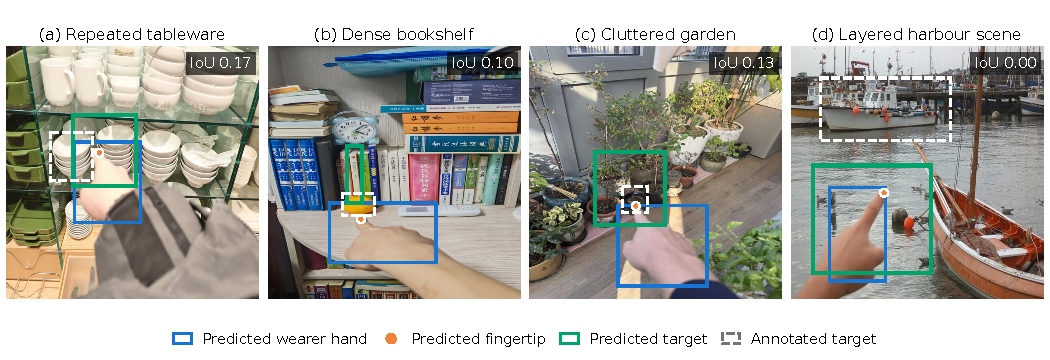
\includegraphics[width=\linewidth]{figures/failures_complex}
  \caption{Selected complex failures: repeated tableware (a) and a dense bookshelf (b) create look-alike neighbours; foliage complicates the target's extent (c); several depth layers separate the fingertip from the labelled boat (d). Colours as in Figure~\ref{fig:teaser}; boxes, points and IoUs are the saved test predictions of the 160\,px model.}
  \Description{Four egocentric photos where the predicted target box misses the labelled one: a box on the wrong stack of tableware in a glass cabinet (IoU 0.17), a box on a neighbouring book in a dense bookshelf (IoU 0.10), a box covering plants around a small object in a garden (IoU 0.13), and a foreground box instead of a distant boat in a harbour (IoU 0.00). The wearer's hand and fingertip are found in all four.}
  \label{fig:failures}
\end{figure}
